\documentclass[main.tex]{subfiles}

\begin{document}

\subsection{Scopo del progetto}

Il progetto è finalizzato alla simulazione del traffico su una città modellizzata come un grafo diretto, ovvero con doppi sensi e sensi unici.
La domanda che ci siamo posti all' inizio della programmazione era se in un qualche modo i sensi unici potessero essere vantaggiosi in alcune condizioni
rispetto ai doppi sensi.
Semplicemente sostituire due corsie alternate con una sola corsia diminuirebbe la superficie della città
e a parità di numero di automobili aumenterebbe la densità e porterebbe sicuramente ad uno svantaggio, quindi nella simulazione
lasciamo all'utente la possibilità di scegliere il numero di corsie dei sensi unici.

\subsection{Modello}

La città è rappresentata come un grafo a griglia, e tramite una probabilità impostata dall'utente è possibile controllare la frazione di sensi unici.
All'inizio della simulazione la matrice di adiacenza è creata e tale probabilità è la probabilità che in fase di creazione un senso alternato diventi senso unico.
In Fig. \ref{fig:1} è rappresentata una città con pochi sensi unici, per mostrare la struttura a griglia.

\begin{figure}[H]
    \centering
    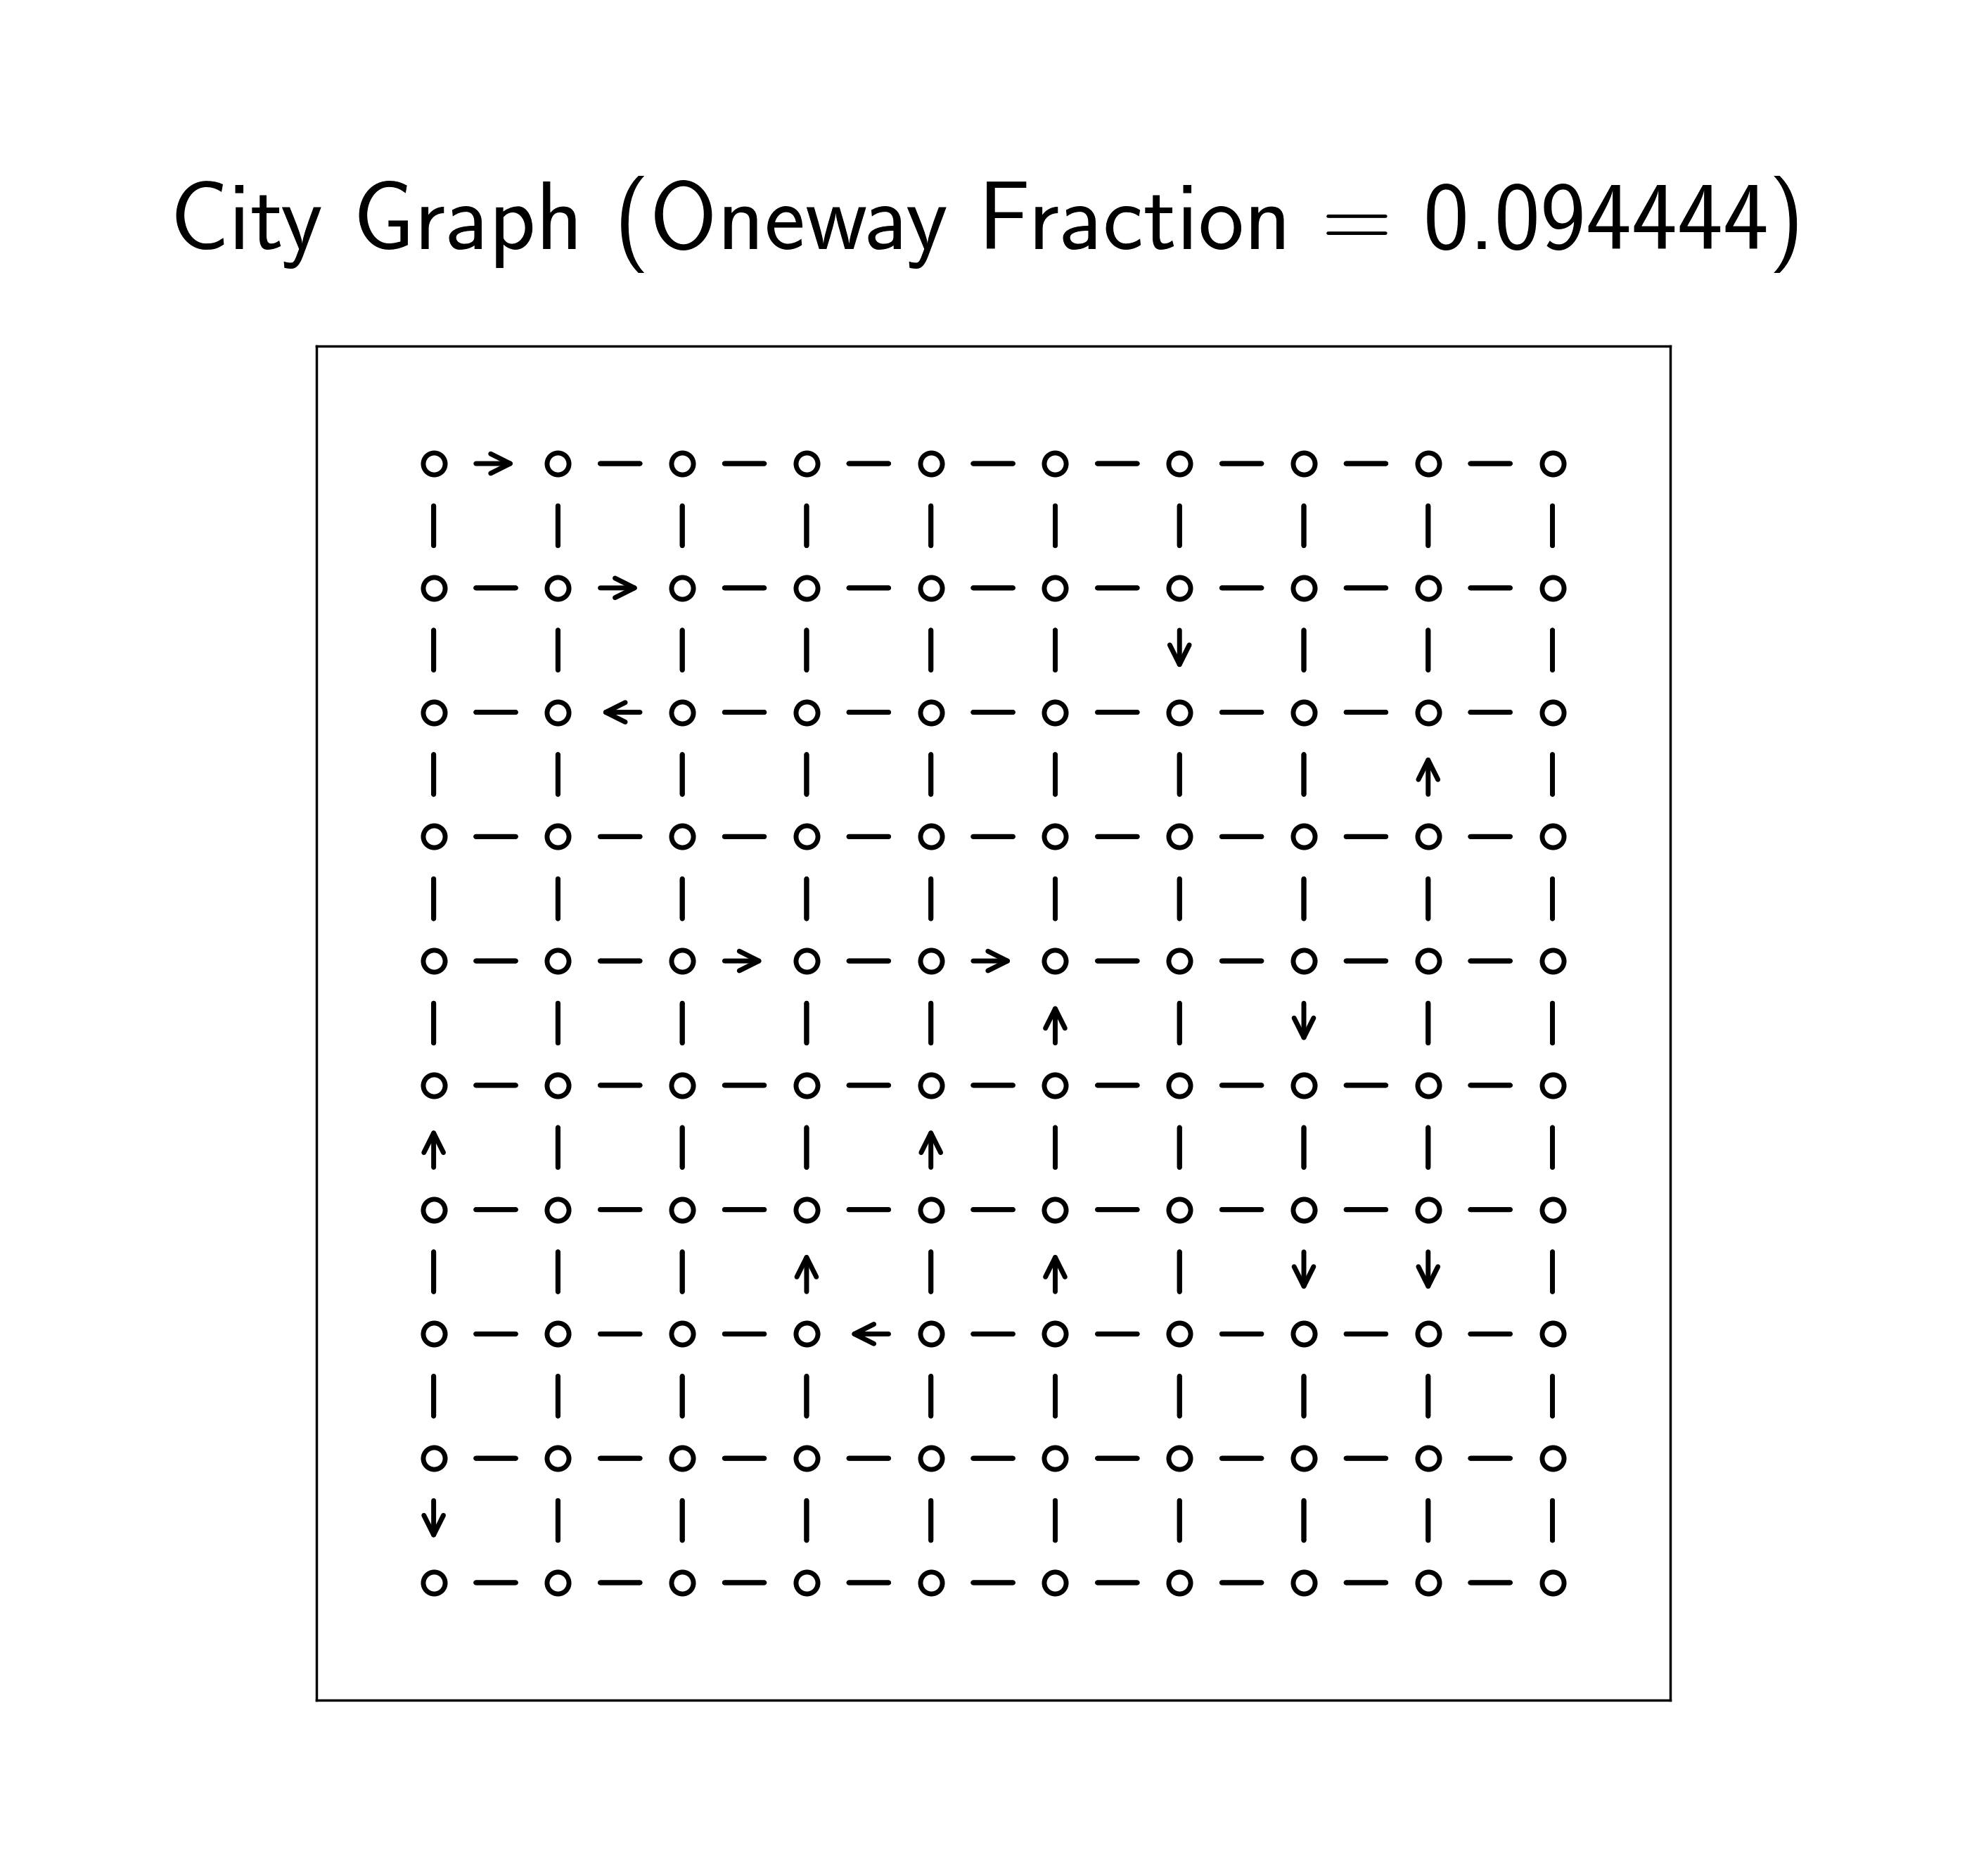
\includegraphics[width=9cm, height=9cm]{city.png}
    \caption{Città a griglia con circa l'1\% di sensi unici.}
    \label{fig:1}
\end{figure}

Può avvenire che l'elevata frazione di sensi unici generi nodi inattraversabili, in Fig. \ref{fig:2} vediamo una strada con molti sensi unici dalla
quale sono stati rimossi i nodi inattraversabili.

\begin{figure}[H]
    \centering
    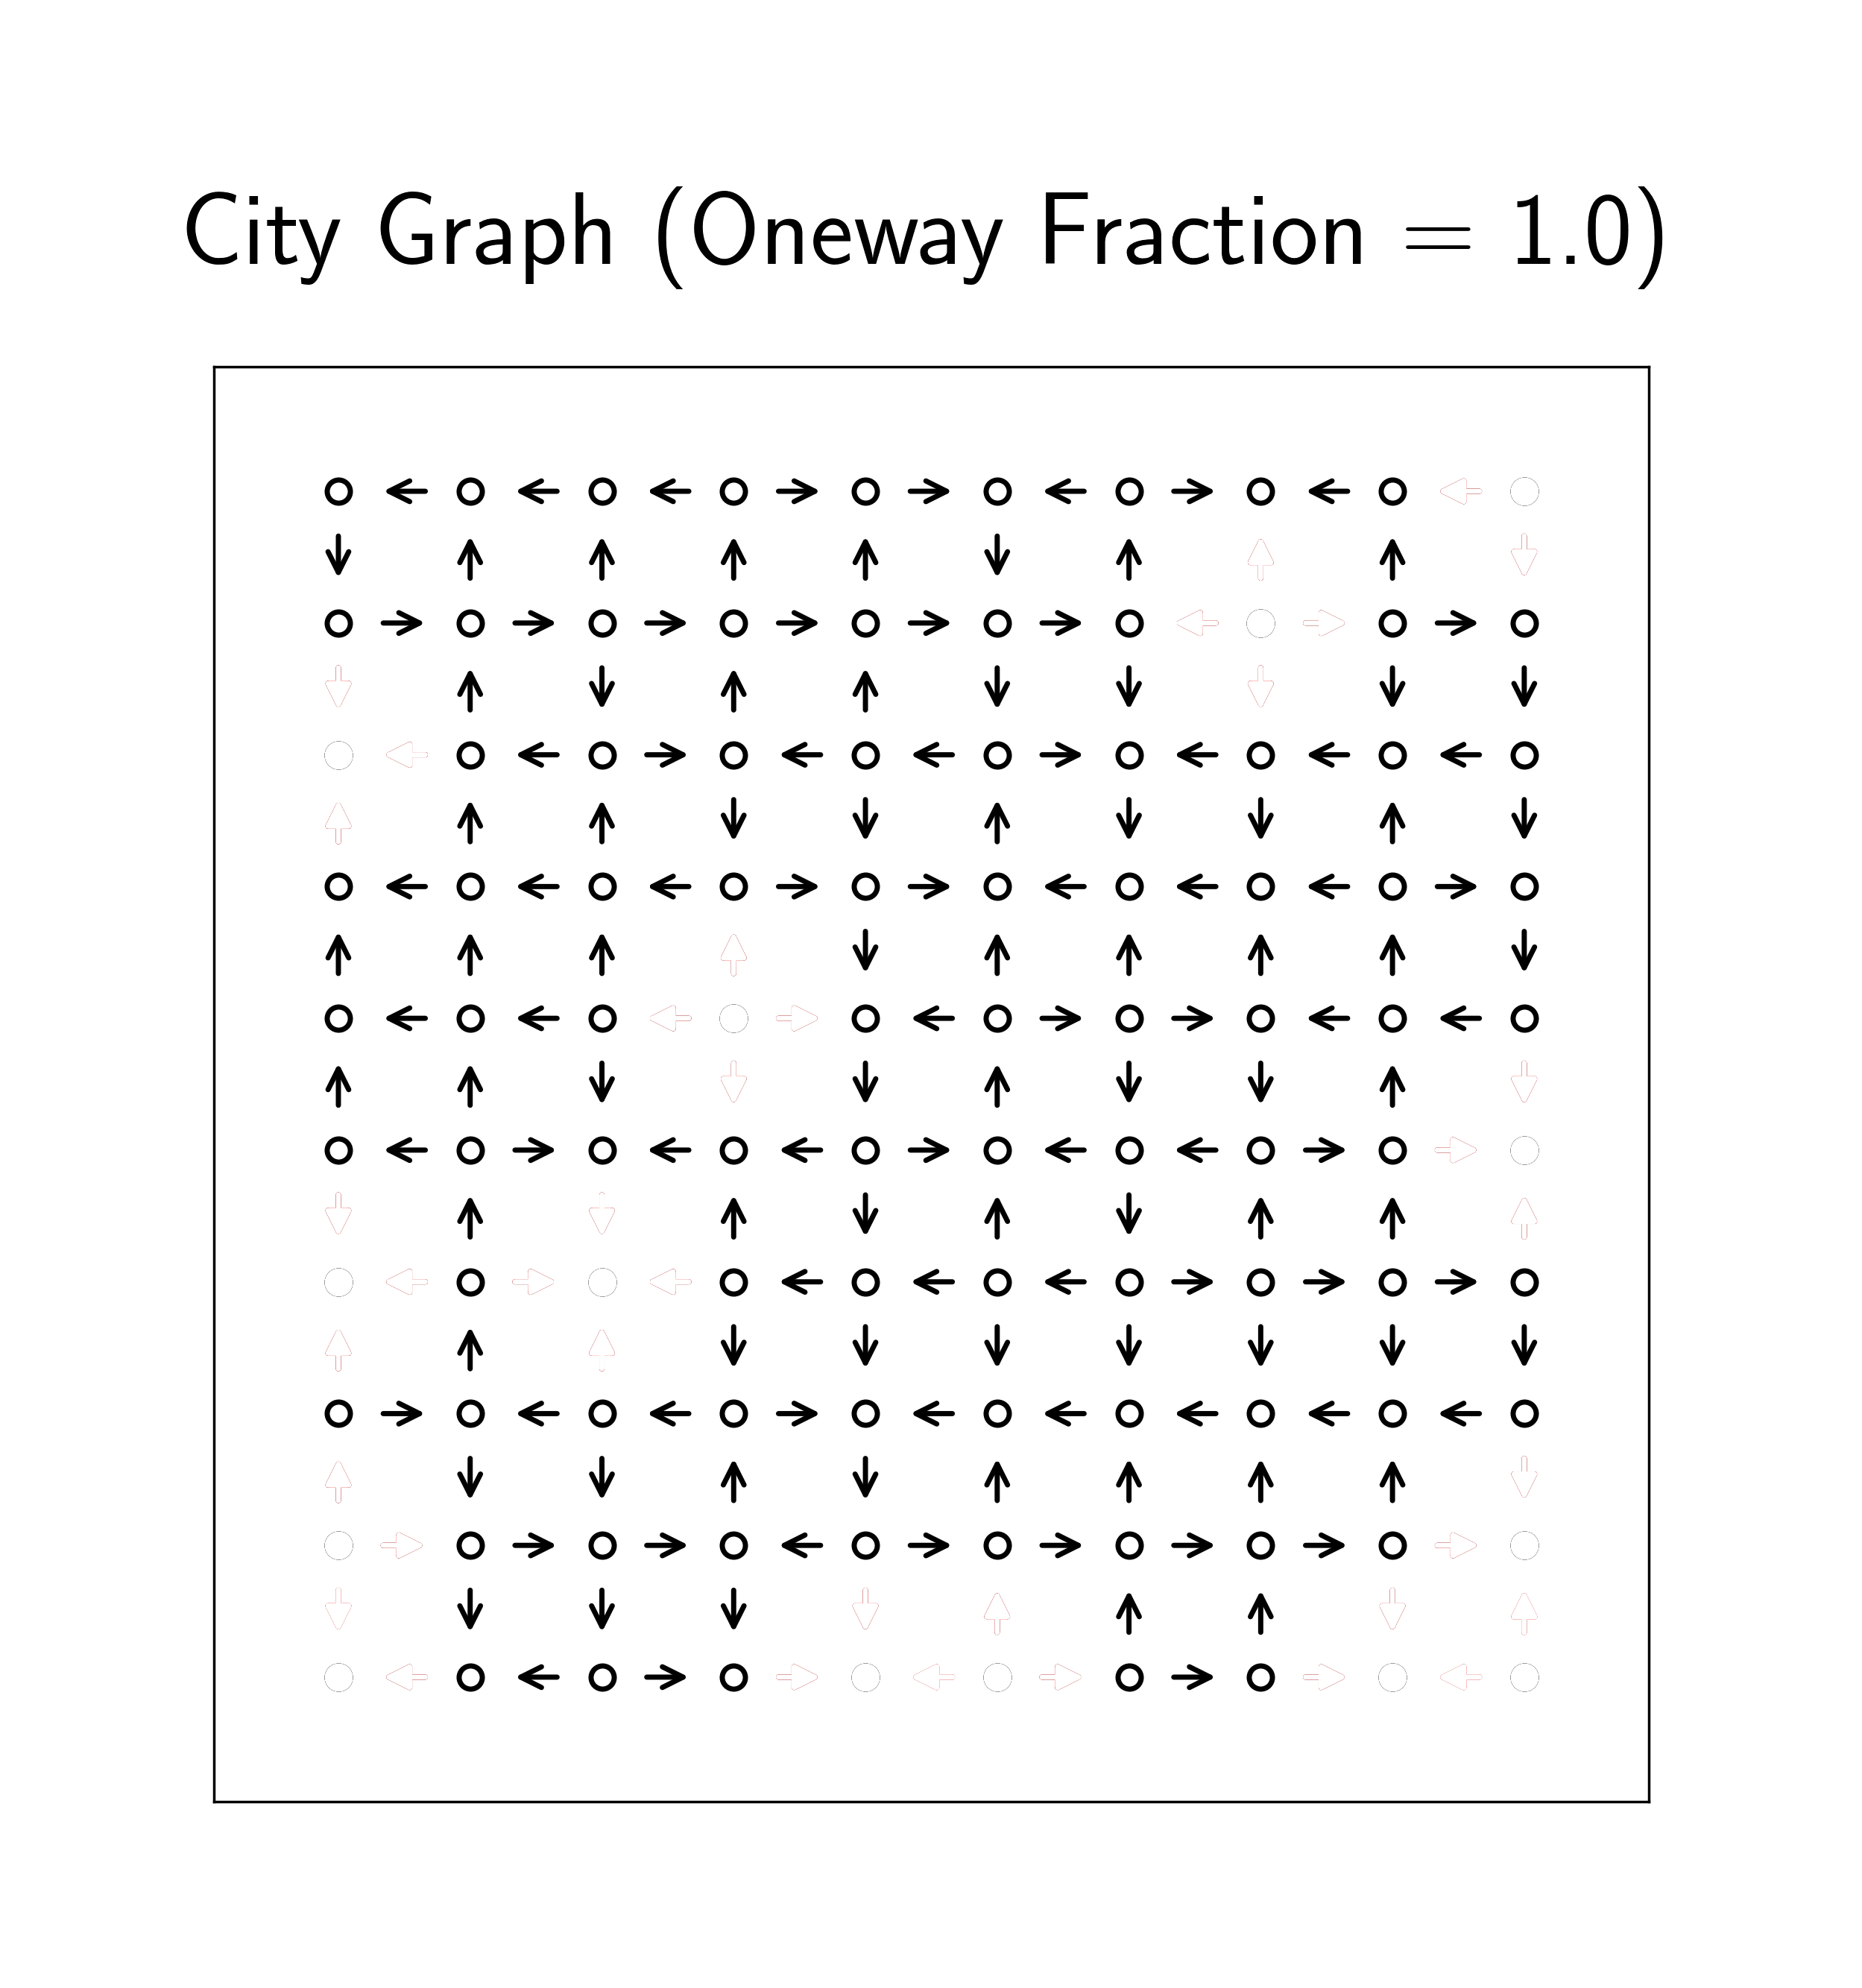
\includegraphics[width=9cm, height=9cm]{city30.png}
    \caption{Città a griglia con soltanto sensi unici.}
    \label{fig:2}
\end{figure}

Notando che in quasi tutte le città con solo sensi unici appariva una struttura simile a quella in Fig. \ref{fig:1}, sulla quale era possibile avere 
percorsi non banali, si è deciso di non mettere controlli per evitare di generare nodi inattraversabili, tale controllo può essere sicuramente aggiunto
negli sviluppi futuri del programma.\\
\hfill \\
Le strade sono modellizzate come dei contenitori di automobili che sanno soltanto il numero di automobili che contengono, però dato che ogni automobile conosce il suo offset sulla strada
questo modello è analogo ad una strada vista come un array in ogni casella del quale è possibile mettere al più un numero di macchine pari al numero di corsie della strada.

In questa simulazione il traffico emerge da un controllo sul movimento delle automobili che impedisce
alla singola automobile di entrare in una casella che contenga un numero di macchine pari al numero di corsie della strada.

Ogni automobile conta il numero di volte in cui passa da una casella a quella successiva e anche il numero di volte in cui
è costretta a fermarsi a causa del traffico.

\subsection{Parametri della Simulazione }

Questo modello ha molti parametri liberi che lo rendono molto flessibile ma possono nascondere effetti che sono osservabili sono in alcuni range di 
tali parametri. 
I parametri sono i seguenti:
\begin{itemize}
    \item \bb{Numero di righe e colonne di nodi}:
        La città è rappresentata come una griglia rettangolare di nodi e l'utente
        può scegliere le dimensioni di questo rettangolo.
    \item \bb{Numero di automobili}
    \item \bb{Numero di corsie dei sensi unici}
    \item \bb{Probabilità di generare un senso unico}:
        Questo parametro permette di controllare a priori la frazione di sensi unici nella città generata.
    \item \bb{Statistiche delle strade}:
        Le lunghezze delle strade sono generate da una distribuzione gaussiana troncata definita dai seguenti parametri.
        \begin{enumerate}[(i)]
            \item Lunghezza massima
            \item Lunghezza minima
            \item Media delle lunghezze
            \item Deviazione standard delle lunghezze
        \end{enumerate}
\end{itemize}

Il parametro di controllo del traffico, nel codice indicato come \ii{traffic index}, è definito come
\[ t =  \frac{\langle p \rangle + \langle s \rangle}{\langle p \rangle}, \]
dove $p$ è il numero di volte in cui l'automobile si è mossa alla casella successiva e $s$ è il numero di volte in cui ha dovuto
fermarsi a causa del traffico.

L'indice di traffico $t$ rappresenta nel nostro modello il rapporto tra i tempi reali di percorrenza e quelli ideali, perciò ci aspettiamo che 
essso sia sempre maggiore o uguale a $1$ e tenda a $1$ diminuendo il numero di auto, come visibile in Fig. \ref{fig:3}.
\end{document}
